\documentclass[pdftex,12pt,a4paper]{article}

\usepackage[turkish,english]{}
\usepackage{graphicx}  
\usepackage[margin=2.5cm]{geometry}
\usepackage{breakcites}
\usepackage{indentfirst}
\usepackage{pgfgantt}
\usepackage{pdflscape}
\usepackage{float}
\usepackage{epsfig}
\usepackage{epstopdf}
\usepackage[cmex10]{amsmath}
\usepackage{url}
\usepackage{stfloats}
\usepackage{multirow}
% \usepackage{karnaugh-map}

\newcommand*\andOp{{\mkern 2mu\cdot\mkern 2mu}}
\renewcommand{\refname}{REFERENCES}

\linespread{1.3}

\usepackage{mathtools}
%\newcommand{\HRule}{\rule{\linewidth}{0.5mm}}
\thispagestyle{empty}
\begin{document}
\begin{titlepage}
\begin{center}
\textbf{}\\
\textbf{\Large{ISTANBUL TECHNICAL UNIVERSITY}}\\
\vspace{0.5cm}
\textbf{\Large{COMPUTER ENGINEERING DEPARTMENT}}\\
\vspace{2cm}
\textbf{\Large{BLG 242E\\ DIGITAL CIRCUITS LABORATORY\\ EXPERIMENT REPORT}}\\
\vspace{2.8cm}
\begin{table}[ht]
\centering
\Large{
\begin{tabular}{lcl}
\textbf{EXPERIMENT NO}  & : & 7 \\
\textbf{EXPERIMENT DATE}  & : & 05.04.2019 \\
\textbf{LAB SESSION}  & : & FRIDAY - 14.00 \\
\textbf{GROUP NO}  & : & G13 \\
\end{tabular}}
\end{table}
\vspace{1cm}
\textbf{\Large{GROUP MEMBERS:}}\\
\begin{table}[ht]
\centering
\Large{
\begin{tabular}{rcl}
{
150180704  & : & C\.{I}HAT AKK\.{I}RAZ \\
150180707  & : & FAT\.{I}H ALTINPINAR \\
150180734  & : & S\.{I}NAN \c{S}AR \\
}
\end{tabular}}
\end{table}
\vspace{2.8cm}
\textbf{\Large{SPRING 2019}}

\end{center}

\end{titlepage}

\newpage

\thispagestyle{empty}
\centering{\LARGE{ \textbf{ETHIC FORM}}}\\
\centering{\LARGE{\textbf{for}}}\\
\centering{\LARGE{\textbf{BLG242E Logic Circuits Laboratory}}}\\[0.2cm]
As a student of \\Istanbul Technical University Faculty of Computer and Informatics Engineering;
\begin{enumerate}
    \item I will not attempt to cheat in quizes and final exam,
    \item I will not use disallowed sources or tools (mobile phone, calculator etc.) during the exam,
    \item I will not write any information (formula, text, figure etc.) on the table, sheets or books that are allowed to be used during the exam,
    \item I will give reference when using printed or online published sources,
    \item I will not use the results in a source as they are, or by changing a part of them without giving a reference,
    \item I will not show unused sources as used, 
    \item I will not present someone else’s idea as my own idea, 
    \item I will not make someone do my homework, project or thesis for money or anything else,
    \item I will not take an exam or enter a lecture on behalf of others,
    \item I will not make excuses for not attending in exams or lessons by taking reports from someone I know (medical doctor parents or relatives),
    \item I will refrain from deliberately harming the public materials at our university,  
    \item I will comply with the safety rules in laboratory work,
    \item I will behave in accordance with the rules of respect for the lecturers and teaching assistants
\end{enumerate}
\vspace{-1em}
\centering{\LARGE{signed by}}\\
\vspace{-1em}
\begin{table}[ht]
\centering
\begin{tabular}{rcl}
150180704  & : & C\.{I}HAT AKK\.{I}RAZ \\
150180707  & : & FAT\.{I}H ALTINPINAR \\
150180734  & : & S\.{I}NAN \c{S}AR \\
\end{tabular}
\end{table}
\vspace{-1em}
 \begin{table}[ht]
 \begin{tabular}{lr}
%\textbf{Date:\hspace*{1.0cm}/\hspace*{1.0cm}/} &\qquad \qquad\qquad\qquad \qquad\qquad\qquad \qquad\qquad\qquad \qquad\qquad \textbf{SIGNED}\\
\end{tabular}
\end{table} % adds the ethic sign
\addcontentsline{toc}{section}{\numberline {}ETHICS}
\newpage

\thispagestyle{empty}
\addtocontents{toc}{\contentsline {section}{\numberline {}FRONT COVER}{}}
\addtocontents{toc}{\contentsline {section}{\numberline {}CONTENTS}{}}
\setcounter{tocdepth}{4}
\tableofcontents
\clearpage

%\begin{figure}[ht]
%	\centering
%	\includegraphics[width=0.5\textwidth]{log%o.png}	
%	\caption{Figure 1}
%	\label{fig1}
%\end{figure}

\setcounter{page}{1}
\section{INTRODUCTION }
\begin{flushleft}
\paragraph{} 
In this experiment series of circuits are built in order to understand how latches, flip flow behave and how to manipulate a signal by a circular shifter.
\end{flushleft}
  

\section{REQUIREMENTS}

\begin{flushleft}
\underline{Tools Used}\cite{booklet}
\end{flushleft}
\begin{itemize}
    \item C.A.D.E.T
    \item 74000 series ICs
    \begin{itemize}
        \item 74$xx^{1}$00 - Quadruple 2-input Positive NAND Gates
        \item 74$xx^{1}$02 - Quadruple 2-input Positive NOR Gates
        \item 74$xx^{1}$04 - Hex Inverters
        \item 74$xx^{1}$75 - Quadruple Bistable D Type Latches
        \item 74$xx^{1}$165 - 8-Bit Parallel Input/Serial Output Shift Register
    \end{itemize}
    \item Oscilloscope
    \item Function Generator
\end{itemize}


\begin{flushleft}
\subsection{PART 1}



\paragraph{}
In this part of the experiment, a S-R latch has to be built with NOR gates. In order to create the base of S-R latch, a stable state needs to be obtained. A stable state can be briefly explained as a circuit that does not oscillate. With the addition of Set and Reset inputs to the leftover inputs of NOR gates, a functioning S-R latch is obtained(see Figure \ref{fig:part1}). As it can be seen in Table \ref{table:part1}, if given zeroes to the inputs of the latch, state remains the same. Set input sets state to 1, reset sets it to 0 as expected. However if high logic applied to both inputs at once, latch loses its stable state and oscillates too fast. Output is observed as 0 in both $Q$ and $\bar{Q}$. Applying 1 to both inputs is forbidden since it makes the circuit unpredictable, yielding different values. Characteristic function of S-R latch can be seen from Table \ref{table:part1}:

\begin{itemize}
    \item $Q(t+1) = S + \bar{R} \cdot Q(t)$
\end{itemize}



\begin{figure}[h]
	\centering
	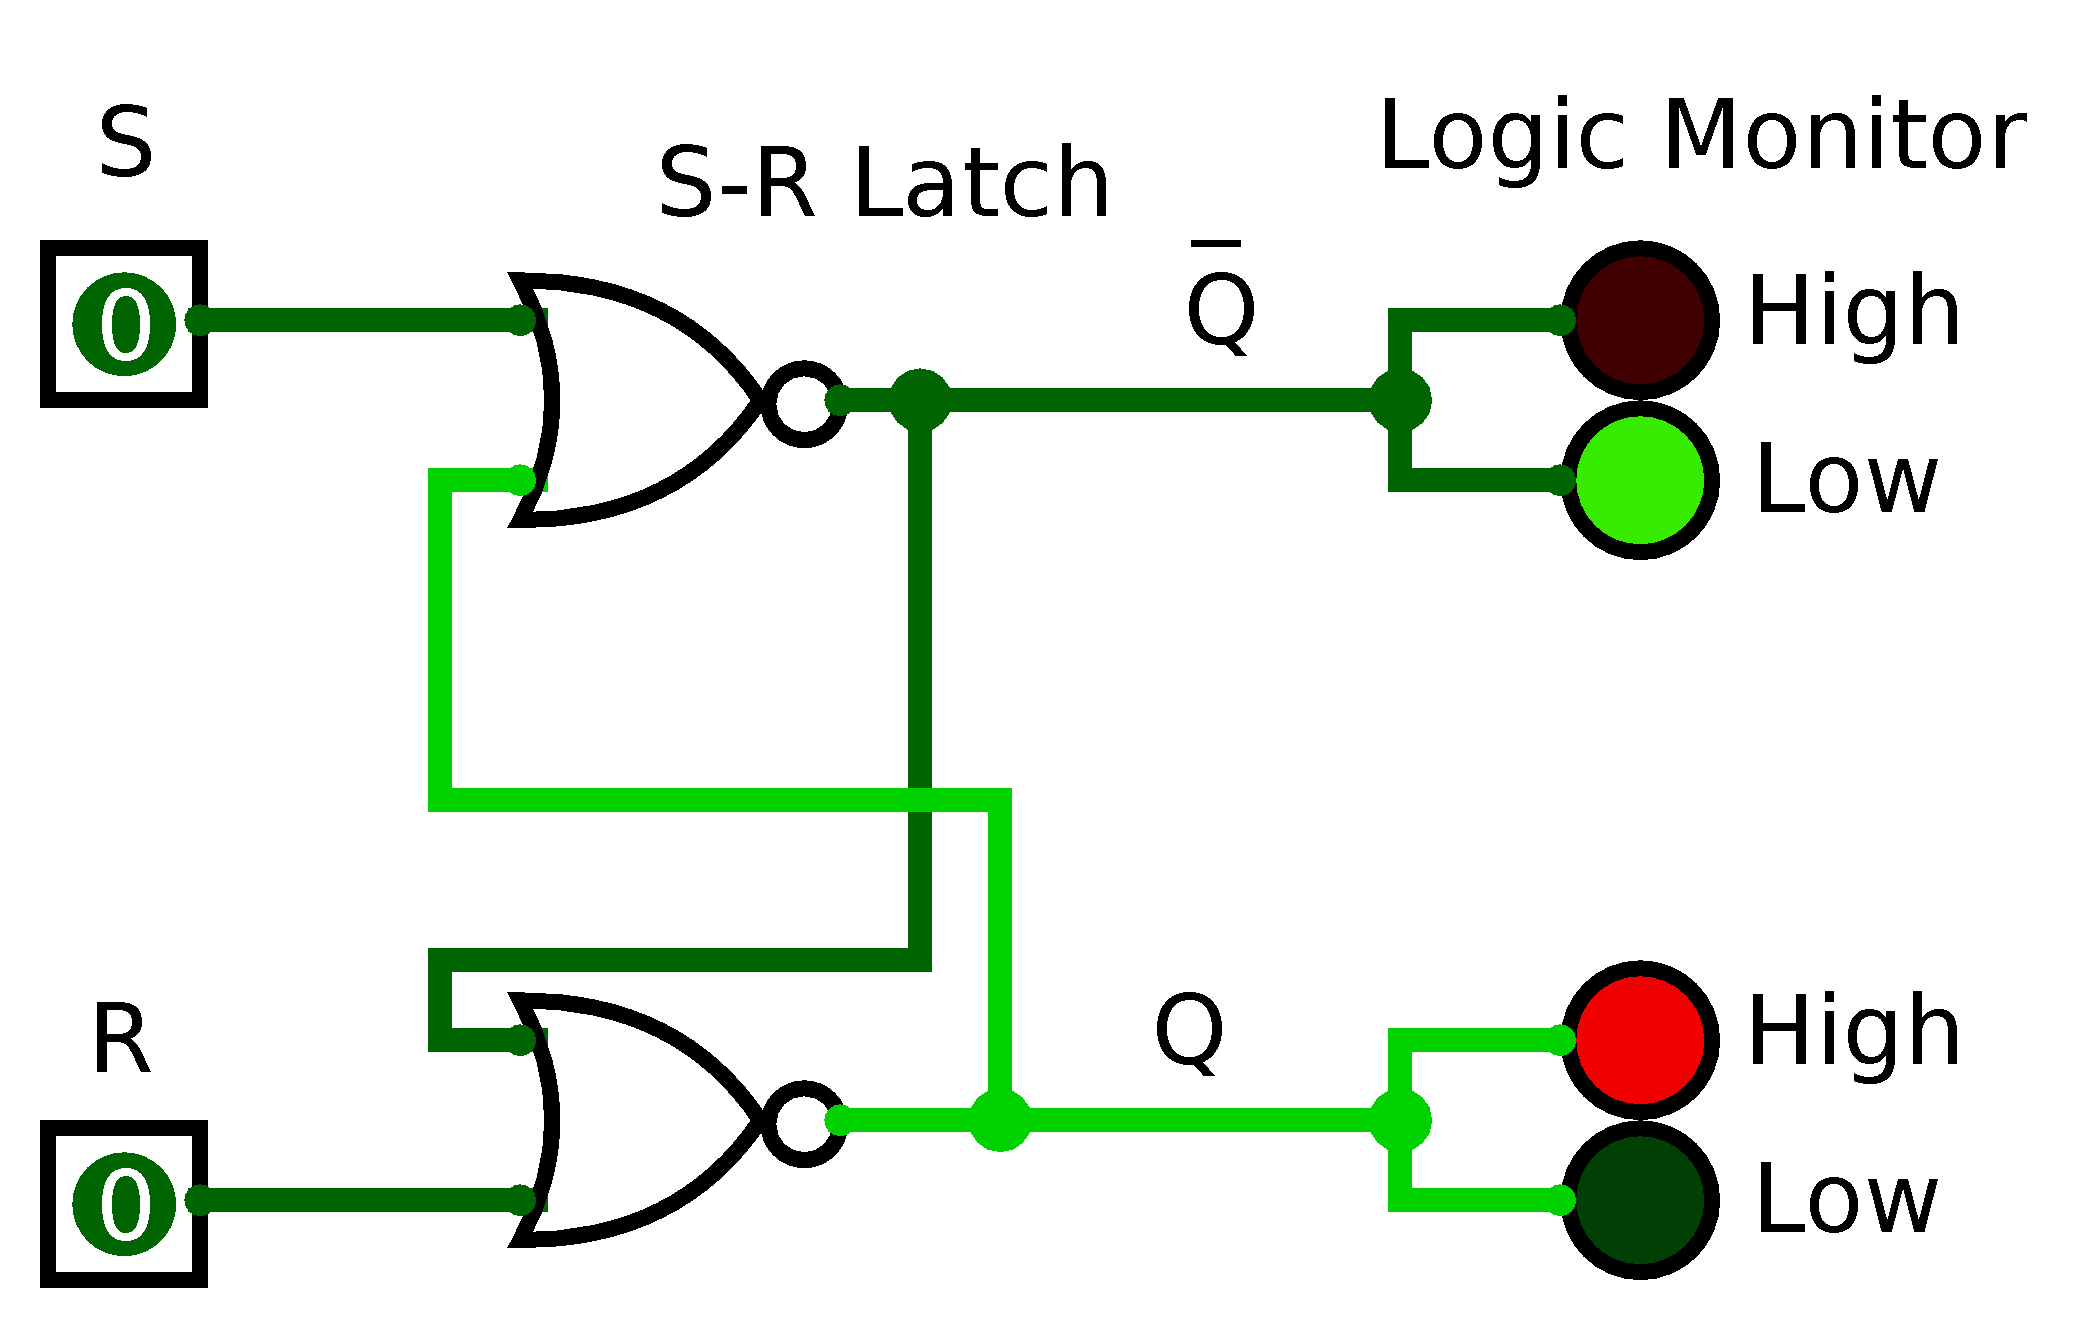
\includegraphics[width=0.5\textwidth]{part1.png}	
	\caption{Circuit of S-R Latch}
	\label{fig:part1}
\end{figure}




\begin{table}[h]
\begin{tabular}{cc|c}
S & R & Q(t+1)                \\ \hline
0 & 0 & Q(t)                \\
0 & 1 & 0                \\
1 & 0 & 1                \\
1 & 1 & $\phi$ Forbidden
\end{tabular}
\centering
\caption{Truth table of S-R Latch}
\label{table:part1}
\end{table}


\end{flushleft}




\begin{flushleft}
\subsection{PART 2}


\begin{figure}[h]
	\centering
	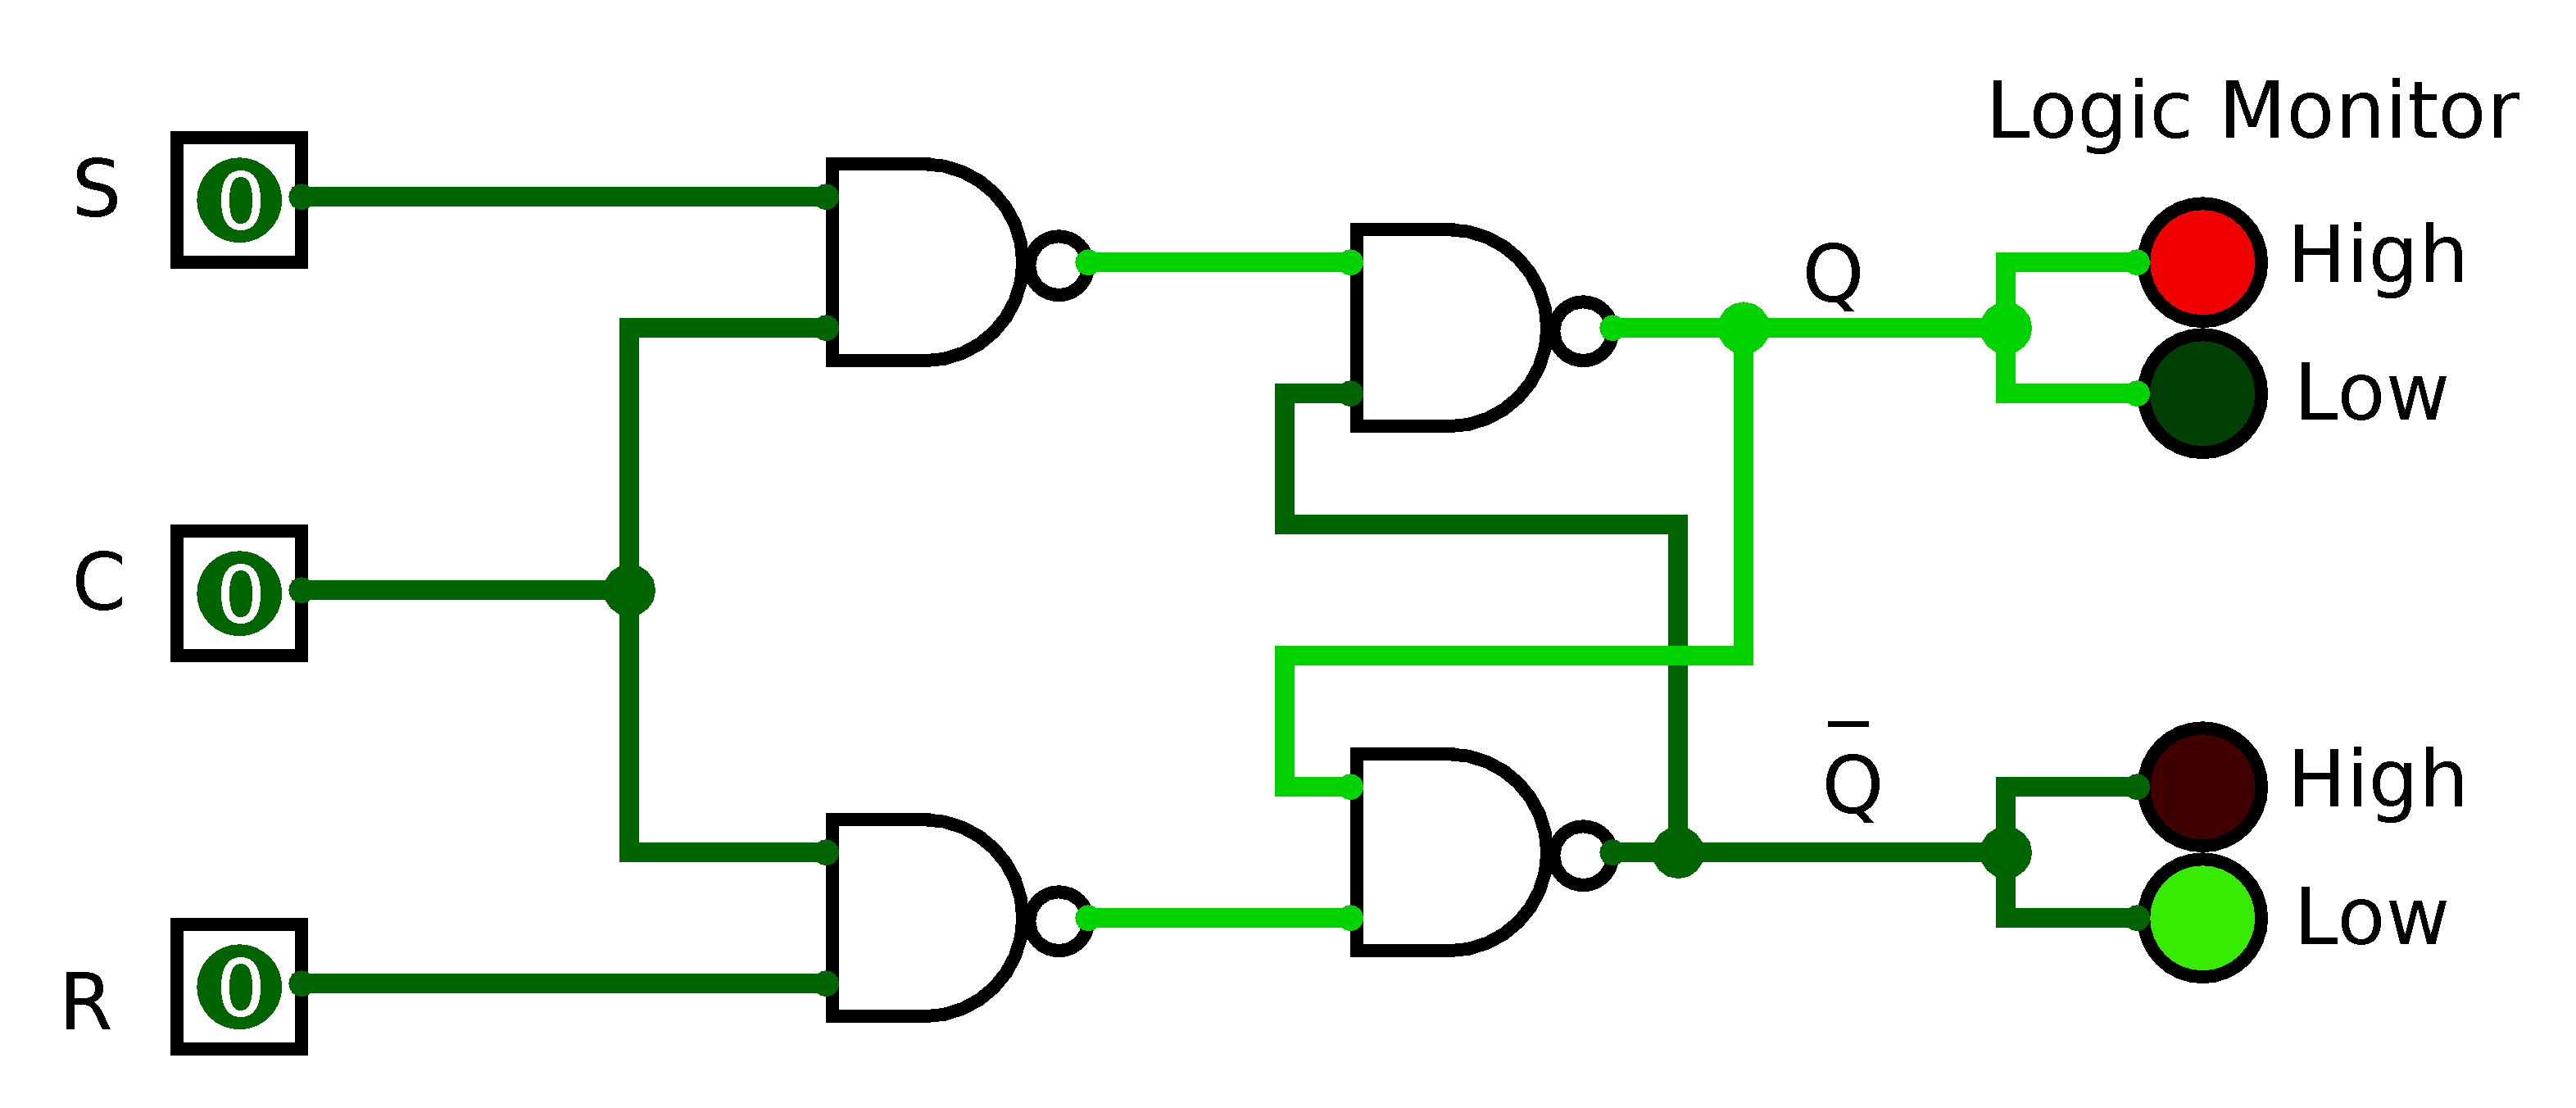
\includegraphics[width=0.5\textwidth]{part2.png}	
	\caption{Circuit of S-R Latch with enable}
	\label{fig:part2}
\end{figure}

\paragraph{}
With the addition of an enable input, another S-R latch is implemented as seen in Figure \ref{fig:part2}. This addition allows S-R latch to change its state only if the enable input is on(high logic state). If given 0 to enable input(C) no change can be observed, otherwise everything is same as it is in Part 1. Except, if given 1 to both Set and Reset inputs to an enabled latch, output is observed on $Q$ and $\bar{Q}$ were 1 rather than zero. This difference is caused by the difference in gates used. The latch is still unpredictable and oscillating very fast. 

\begin{table}[h]
\begin{tabular}{ccc|c}
C & S & R & Q(t+1)           \\ \hline
0 & X & X & Q(t)             \\
1 & 0 & 0 & Q(t)             \\
1 & 0 & 1 & 0                \\
1 & 1 & 0 & 1                \\
1 & 1 & 1 & $\phi$ Forbidden
\end{tabular}
\centering
\caption{Truth table of S-R Latch with enable}
\label{table:part2}
\end{table}



\end{flushleft}



\newpage
\begin{flushleft}
\subsection{PART 3}

\begin{figure}[h]
	\centering
	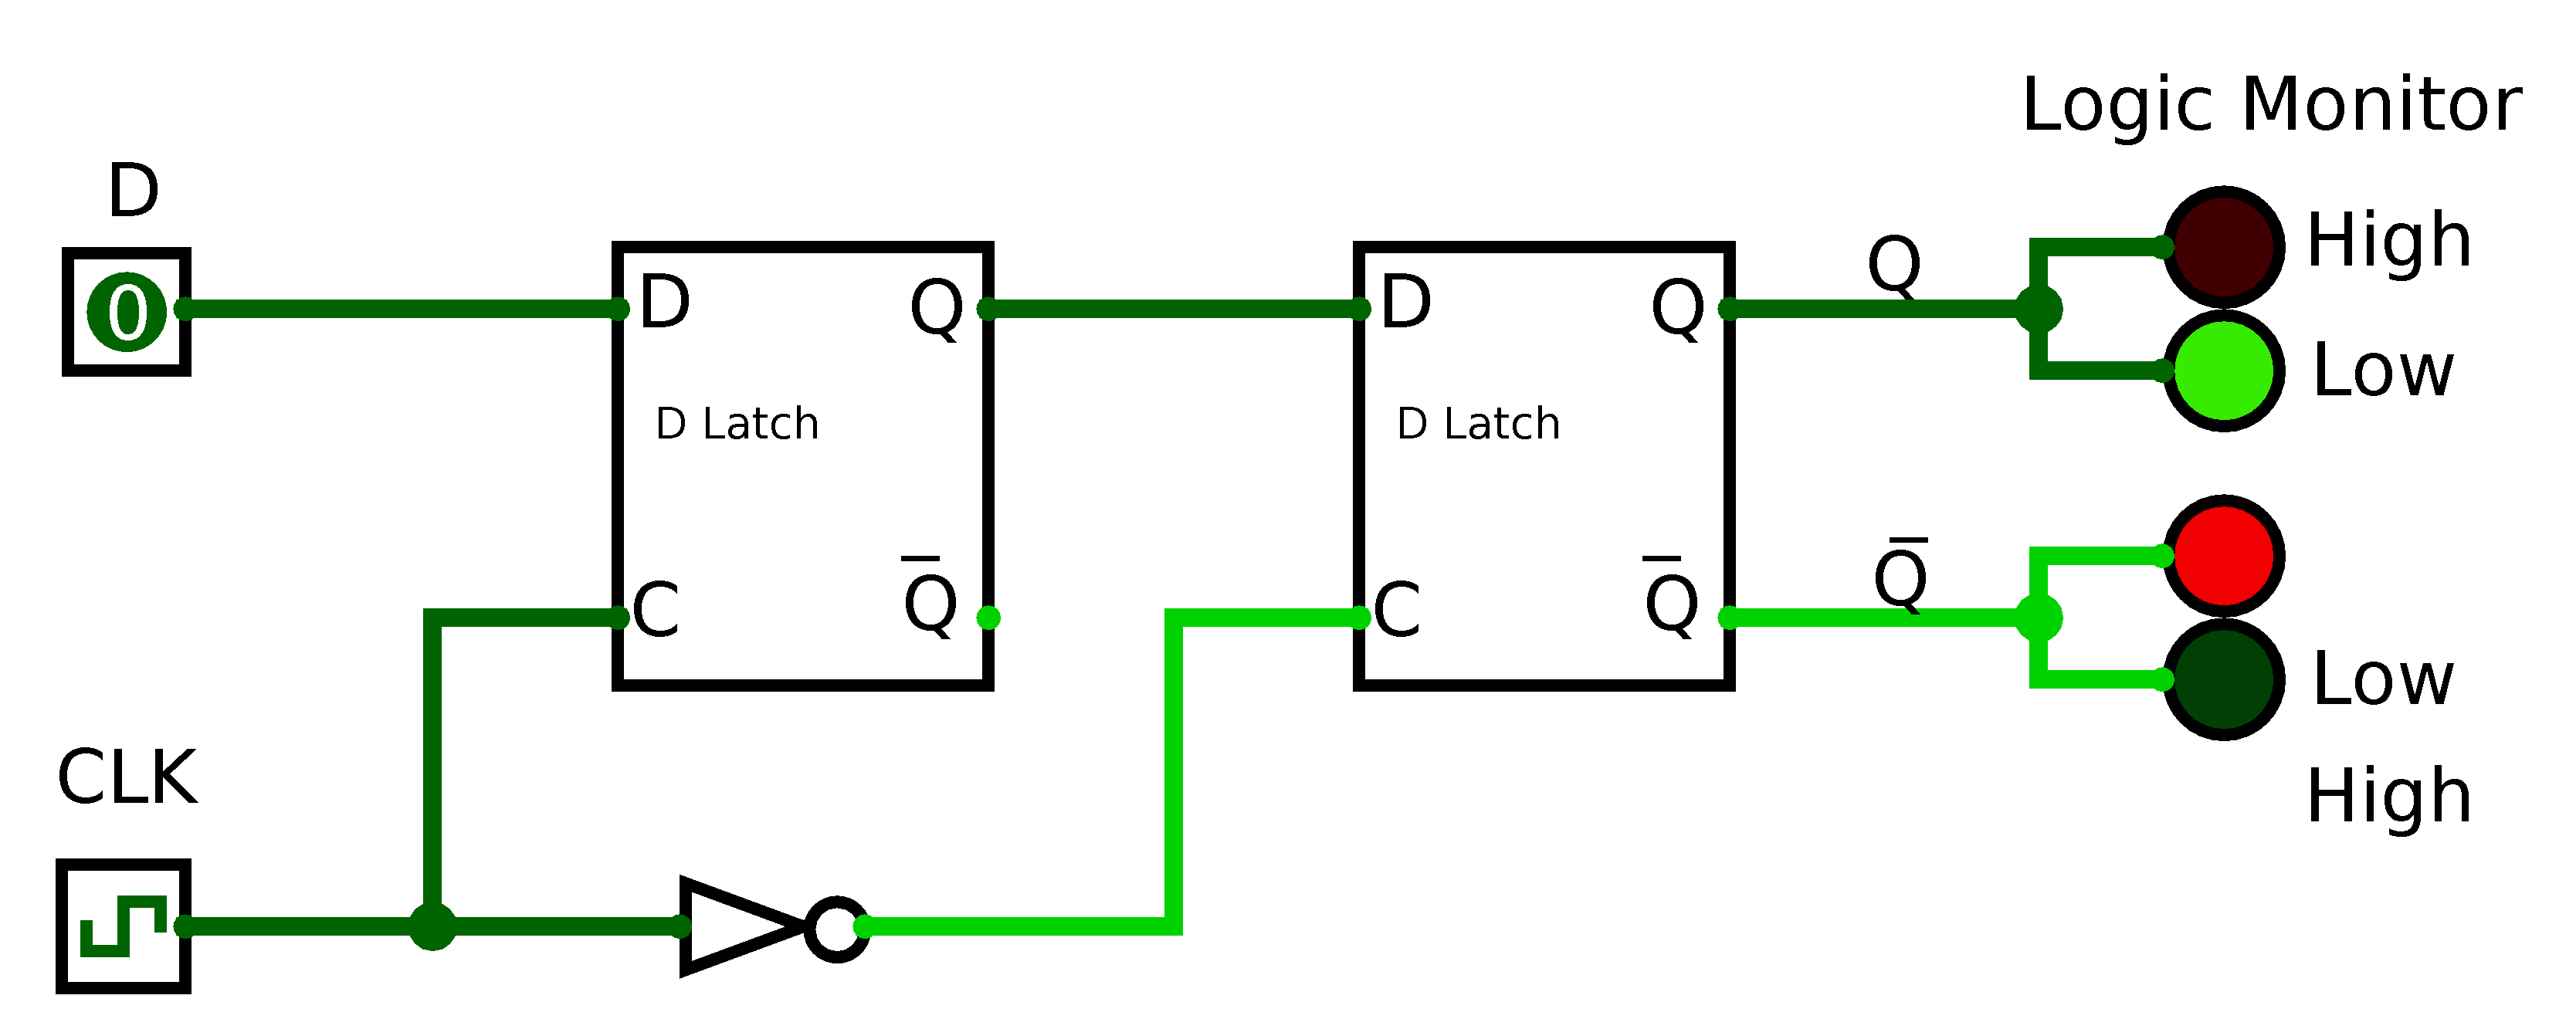
\includegraphics[width=0.5\textwidth]{part3.png}	
	\caption{Circuit of falling edge D flip-flop}
	\label{fig:part3}
\end{figure}

\paragraph{}
In this part, a D type flip flop is constructed (see Figure \ref{fig:part3}), using D type latches. D type latch is a latch that has the characteristic function $Q = D$ if the latch is enabled, otherwise it keeps its state. As it can be seen in Table \ref{table:part3}, state only changes when clock is changing from a high state to low state. Which makes this circuit, a falling edge flip flop.


\begin{table}[h]
\begin{tabular}{cc|c}
D & CLK        & Q(t+1) \\ \hline
0 & $\downarrow$ & 0      \\
1 & $\downarrow$ & 1      \\
x & 0          & Q(t)   \\
x & $\uparrow$   & Q(t)   \\
x & 1          & Q(t)  
\end{tabular}
\centering
\caption{Truth table of falling edge D flip-flop}
\label{table:part3}
\end{table}


\end{flushleft}


\newpage
\begin{flushleft}
\subsection{PART 4}

\begin{figure}[h]
	\centering
	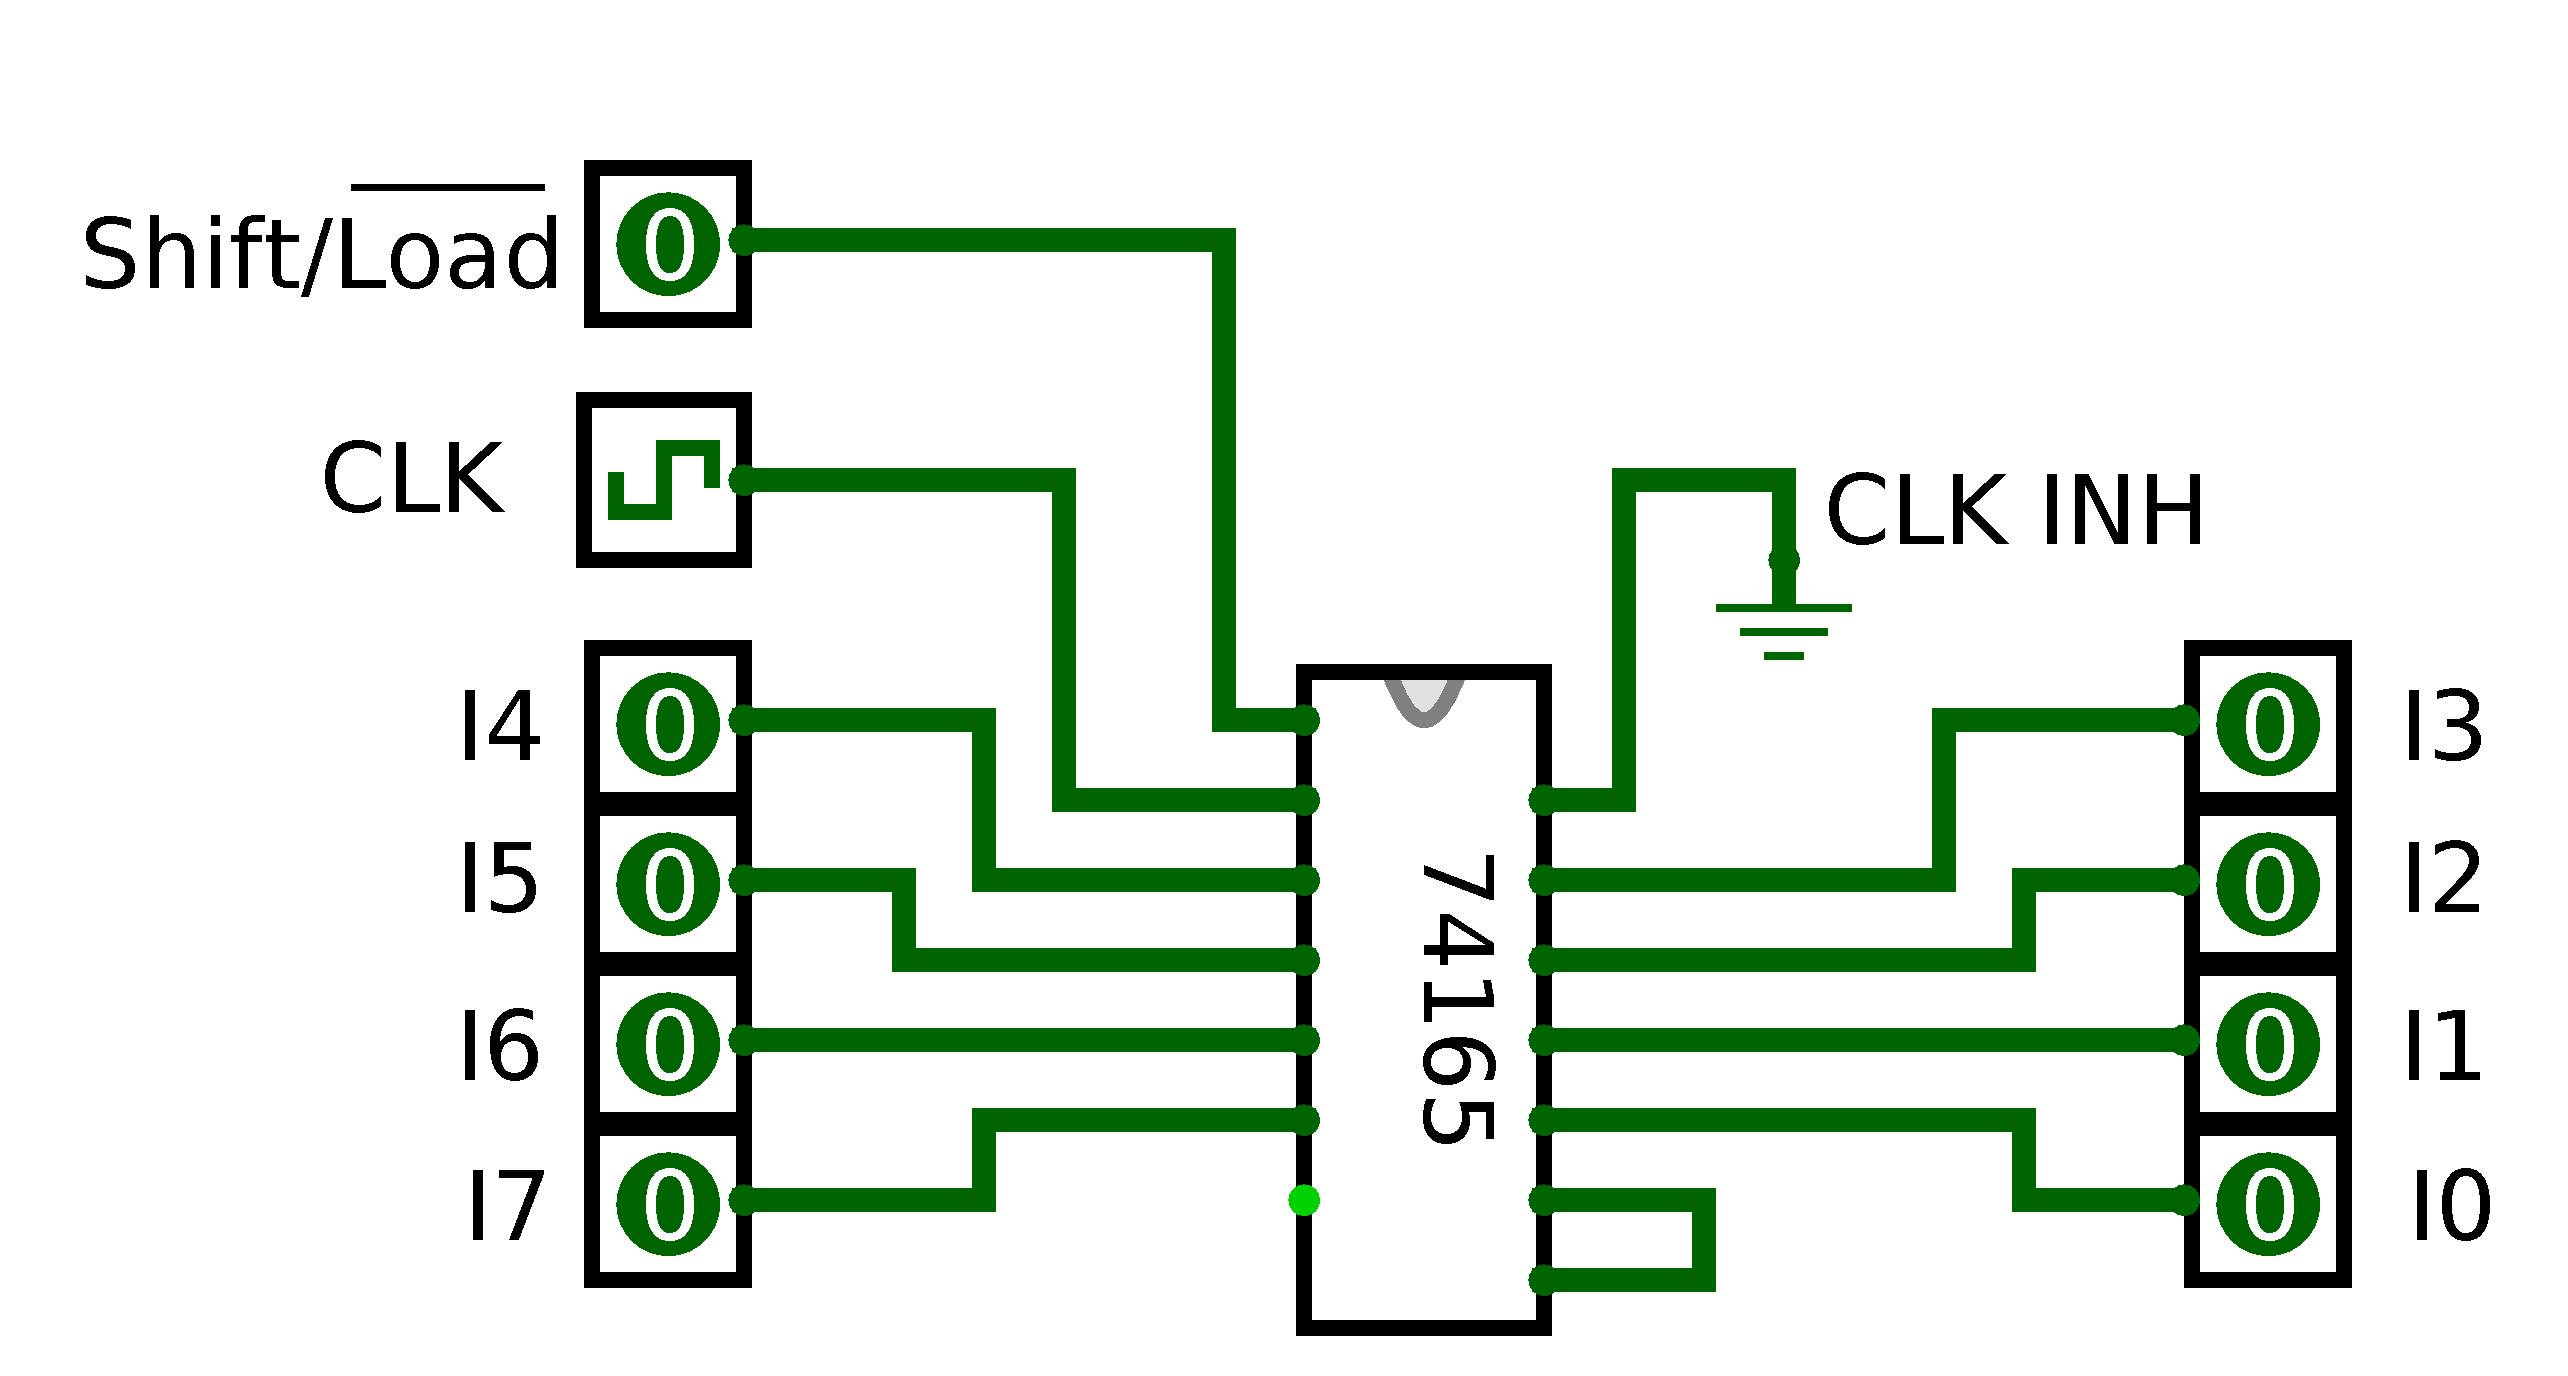
\includegraphics[width=0.5\textwidth]{part4.png}	
	\caption{Circuit built to manipulate input signal}
	\label{fig:part4}
\end{figure}

\paragraph{}
In the final part of the experiment, pulse generator is implemented using a shift register. $Q_{H}$ output of the shift register (bit that is shifted out from $I_{7}$) is connected to $SER$(new value of $I_{0}$).Results are observed for different frequency values and pulse/gap duration rates using the oscilloscope provided in the laboratory. As input, 8 kHz square wave is used since register have 8 bits. This produced nicer graphs in oscilloscope. 

\paragraph{}
In every figure, blue wave is the 8 kHz signal that is produced by signal generator, yellow is the signal that is changed by the shift register.
\paragraph{}
To obtain 1/2 frequency from the input signal, 10101010 bits are loaded to the shift register. Output of the signal can be seen in Figure \ref{fig:1over2}. In the Figure, a single, full cycle of the wave that is produced by the register is as long as 2 full cycles of the wave that is produced by the signal generator. This shows yellow wave has 2 times of the wavelength of blue wave.   
\begin{figure}[h]
	\centering
	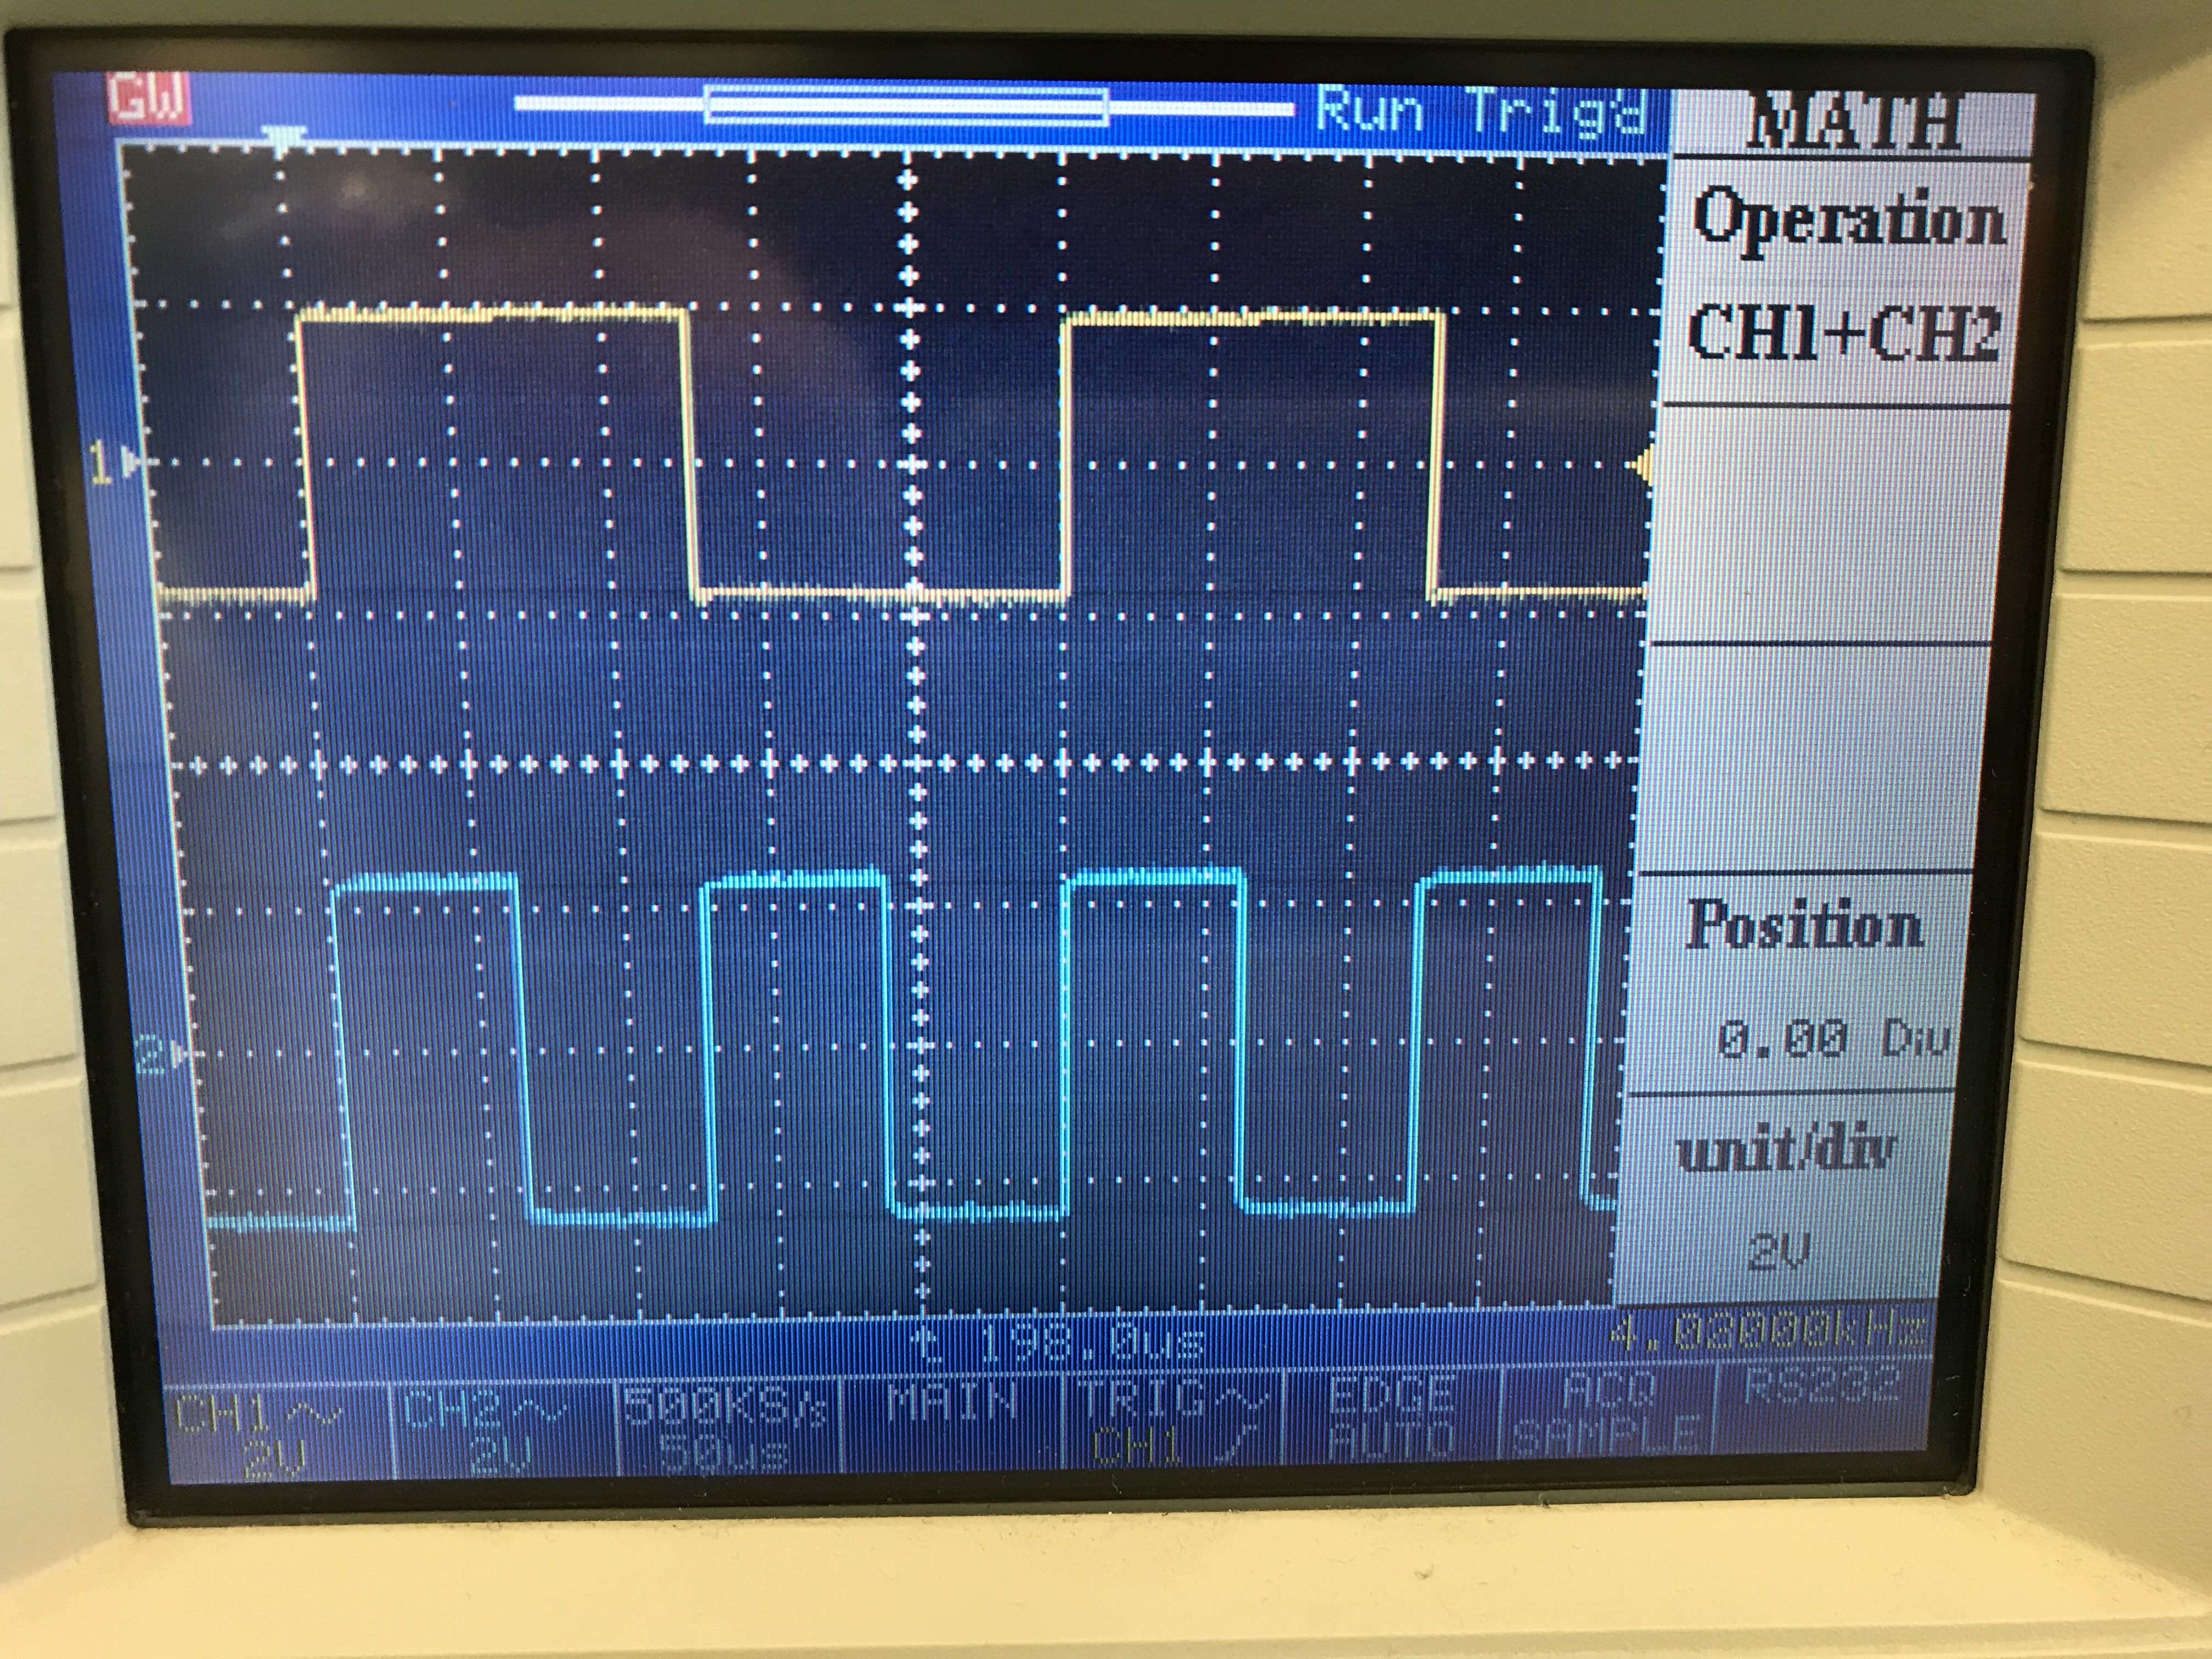
\includegraphics[width=0.5\textwidth]{1over2.jpg}	
	\caption{1/2 frequency of input}
	\label{fig:1over2}
\end{figure}

\paragraph{}
To obtain 1/4 frequency from the input signal, 11001100 bits are loaded to the shift register. Output of the signal can be seen in Figure \ref{fig:1over4}. As it can be counted from the figure, a full cycle of the yellow wave is as long as 4 blue cycles.
\begin{figure}[h]
	\centering
	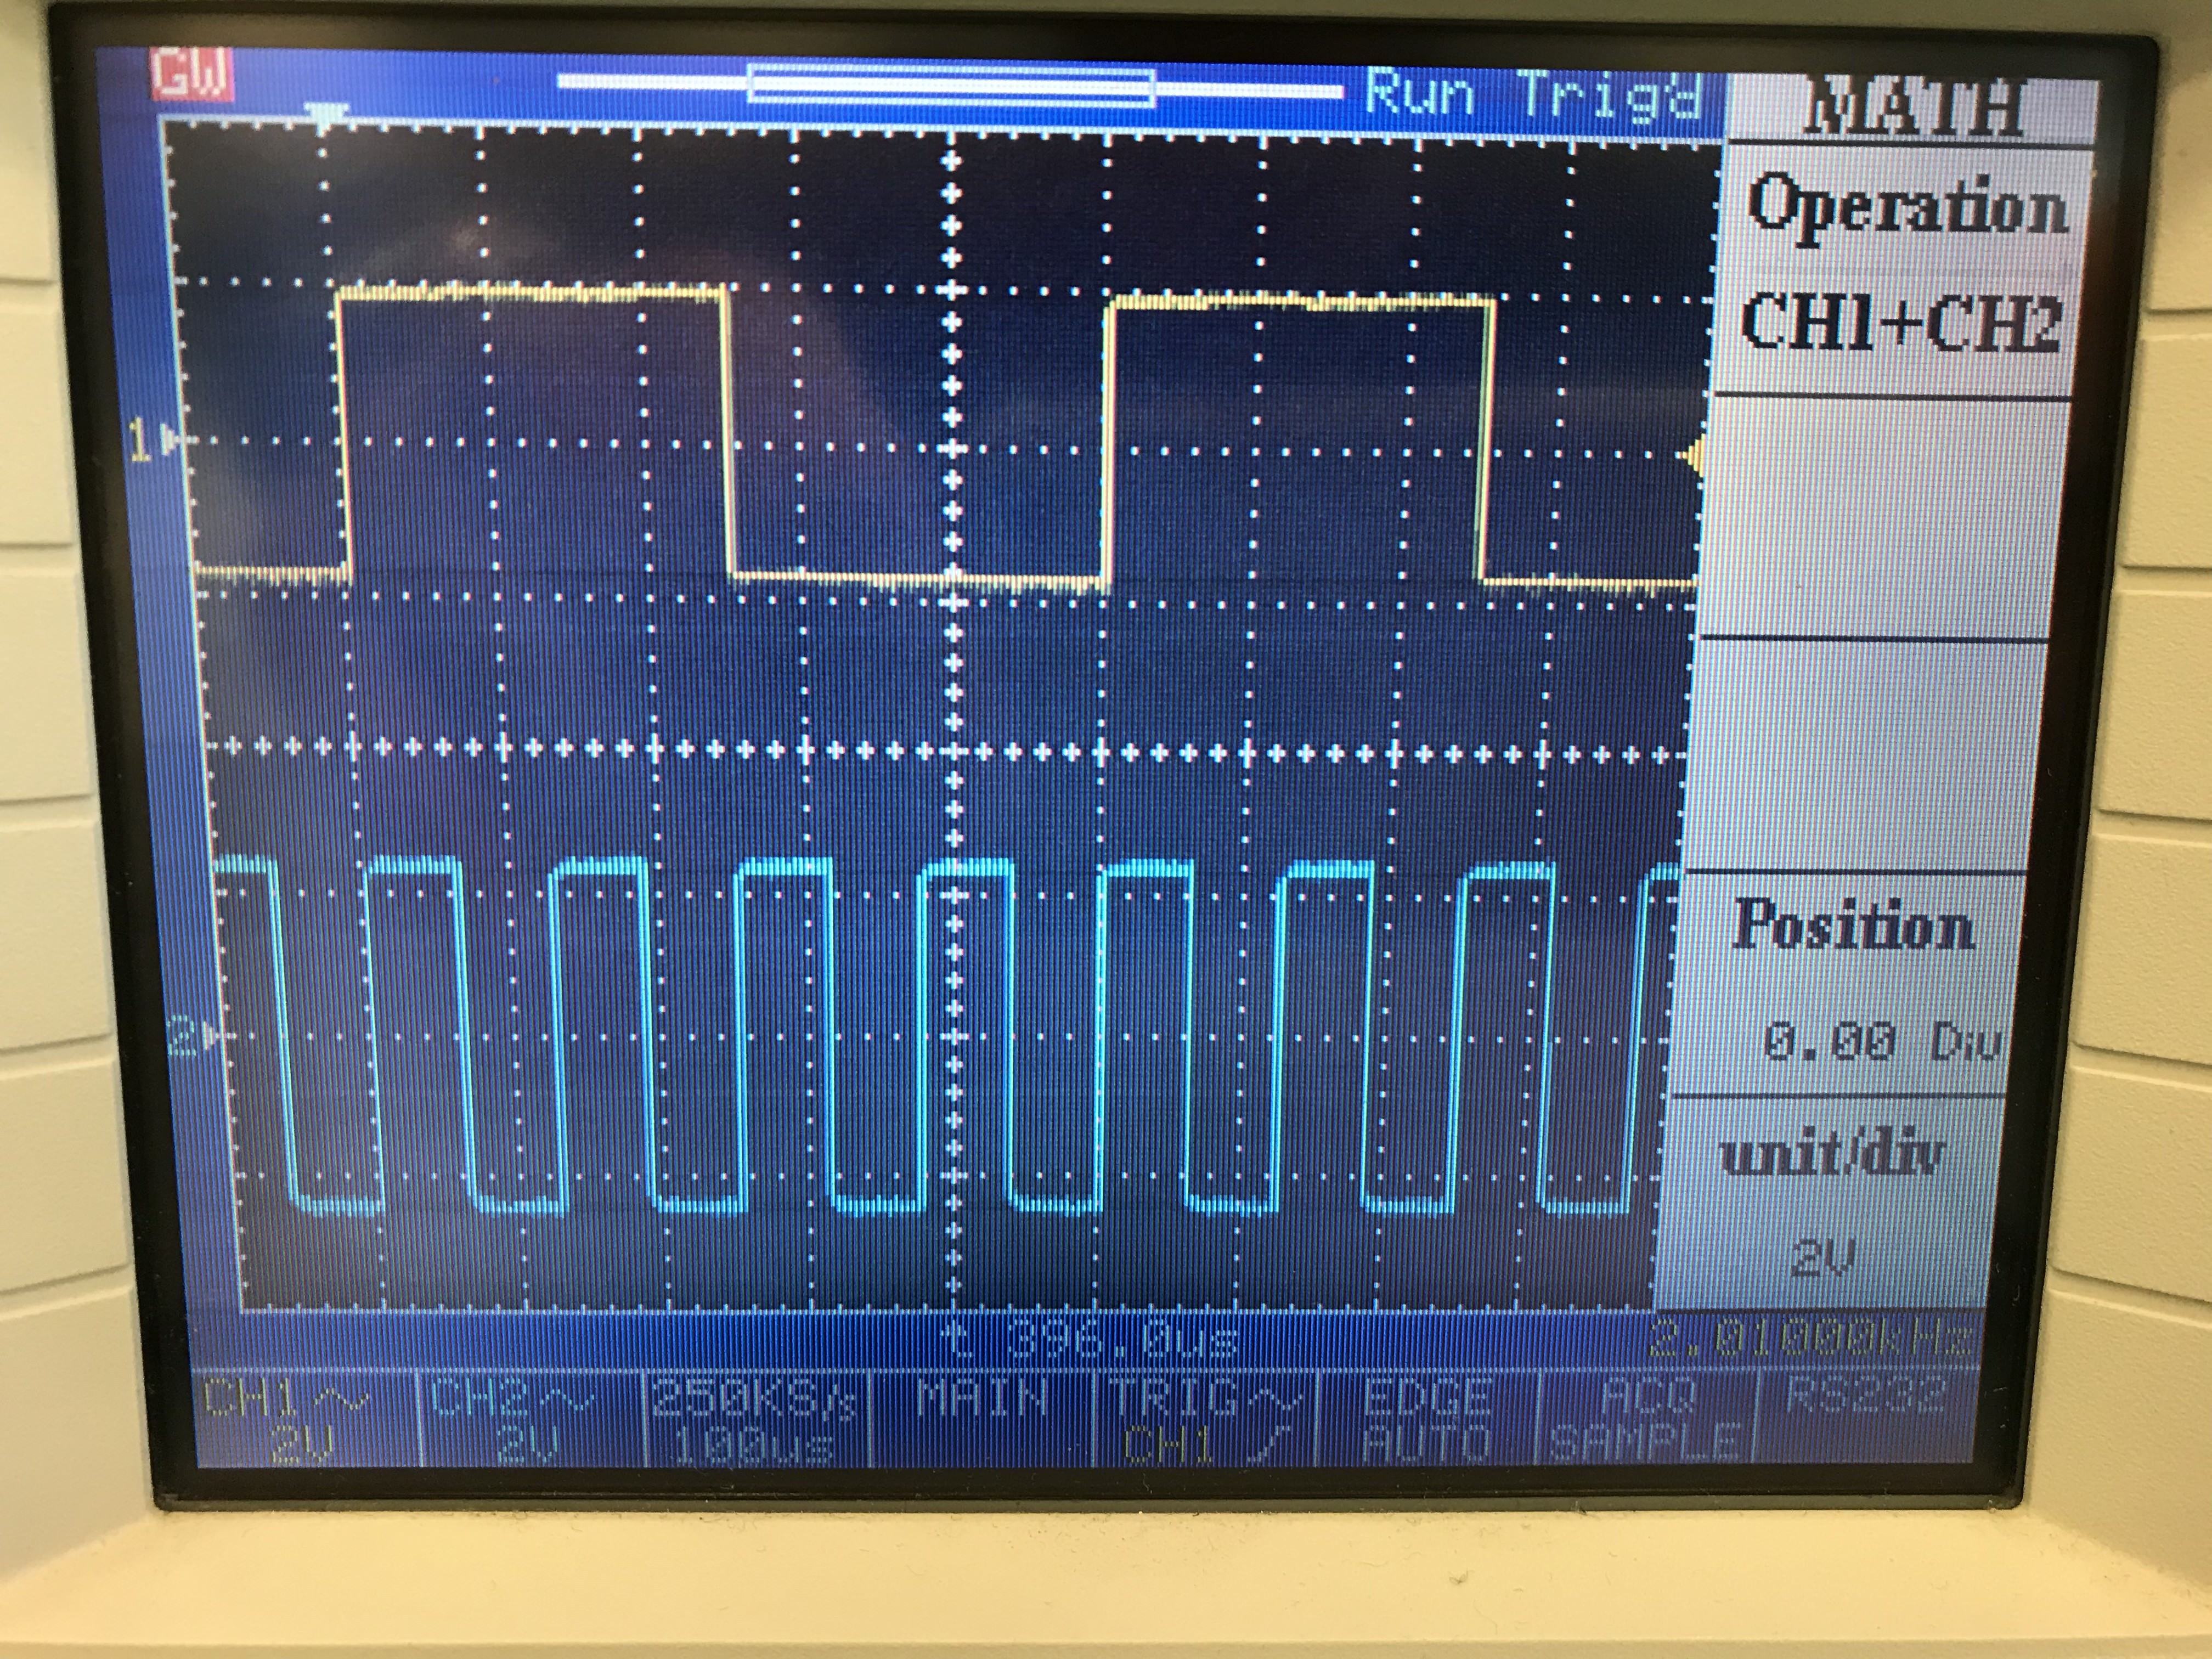
\includegraphics[width=0.5\textwidth]{1over4.jpg}	
	\caption{1/4 frequency of input}
	\label{fig:1over4}
\end{figure}

\paragraph{}
In order to obtain 1/8 frequency from the input signal, 11110000 bits are loaded to the shift register. From the Figure \ref{fig:1over8}, it is clear that, yellow wave's wavelength is 8 times the wavelength of the blue signal.
\begin{figure}[h]
	\centering
	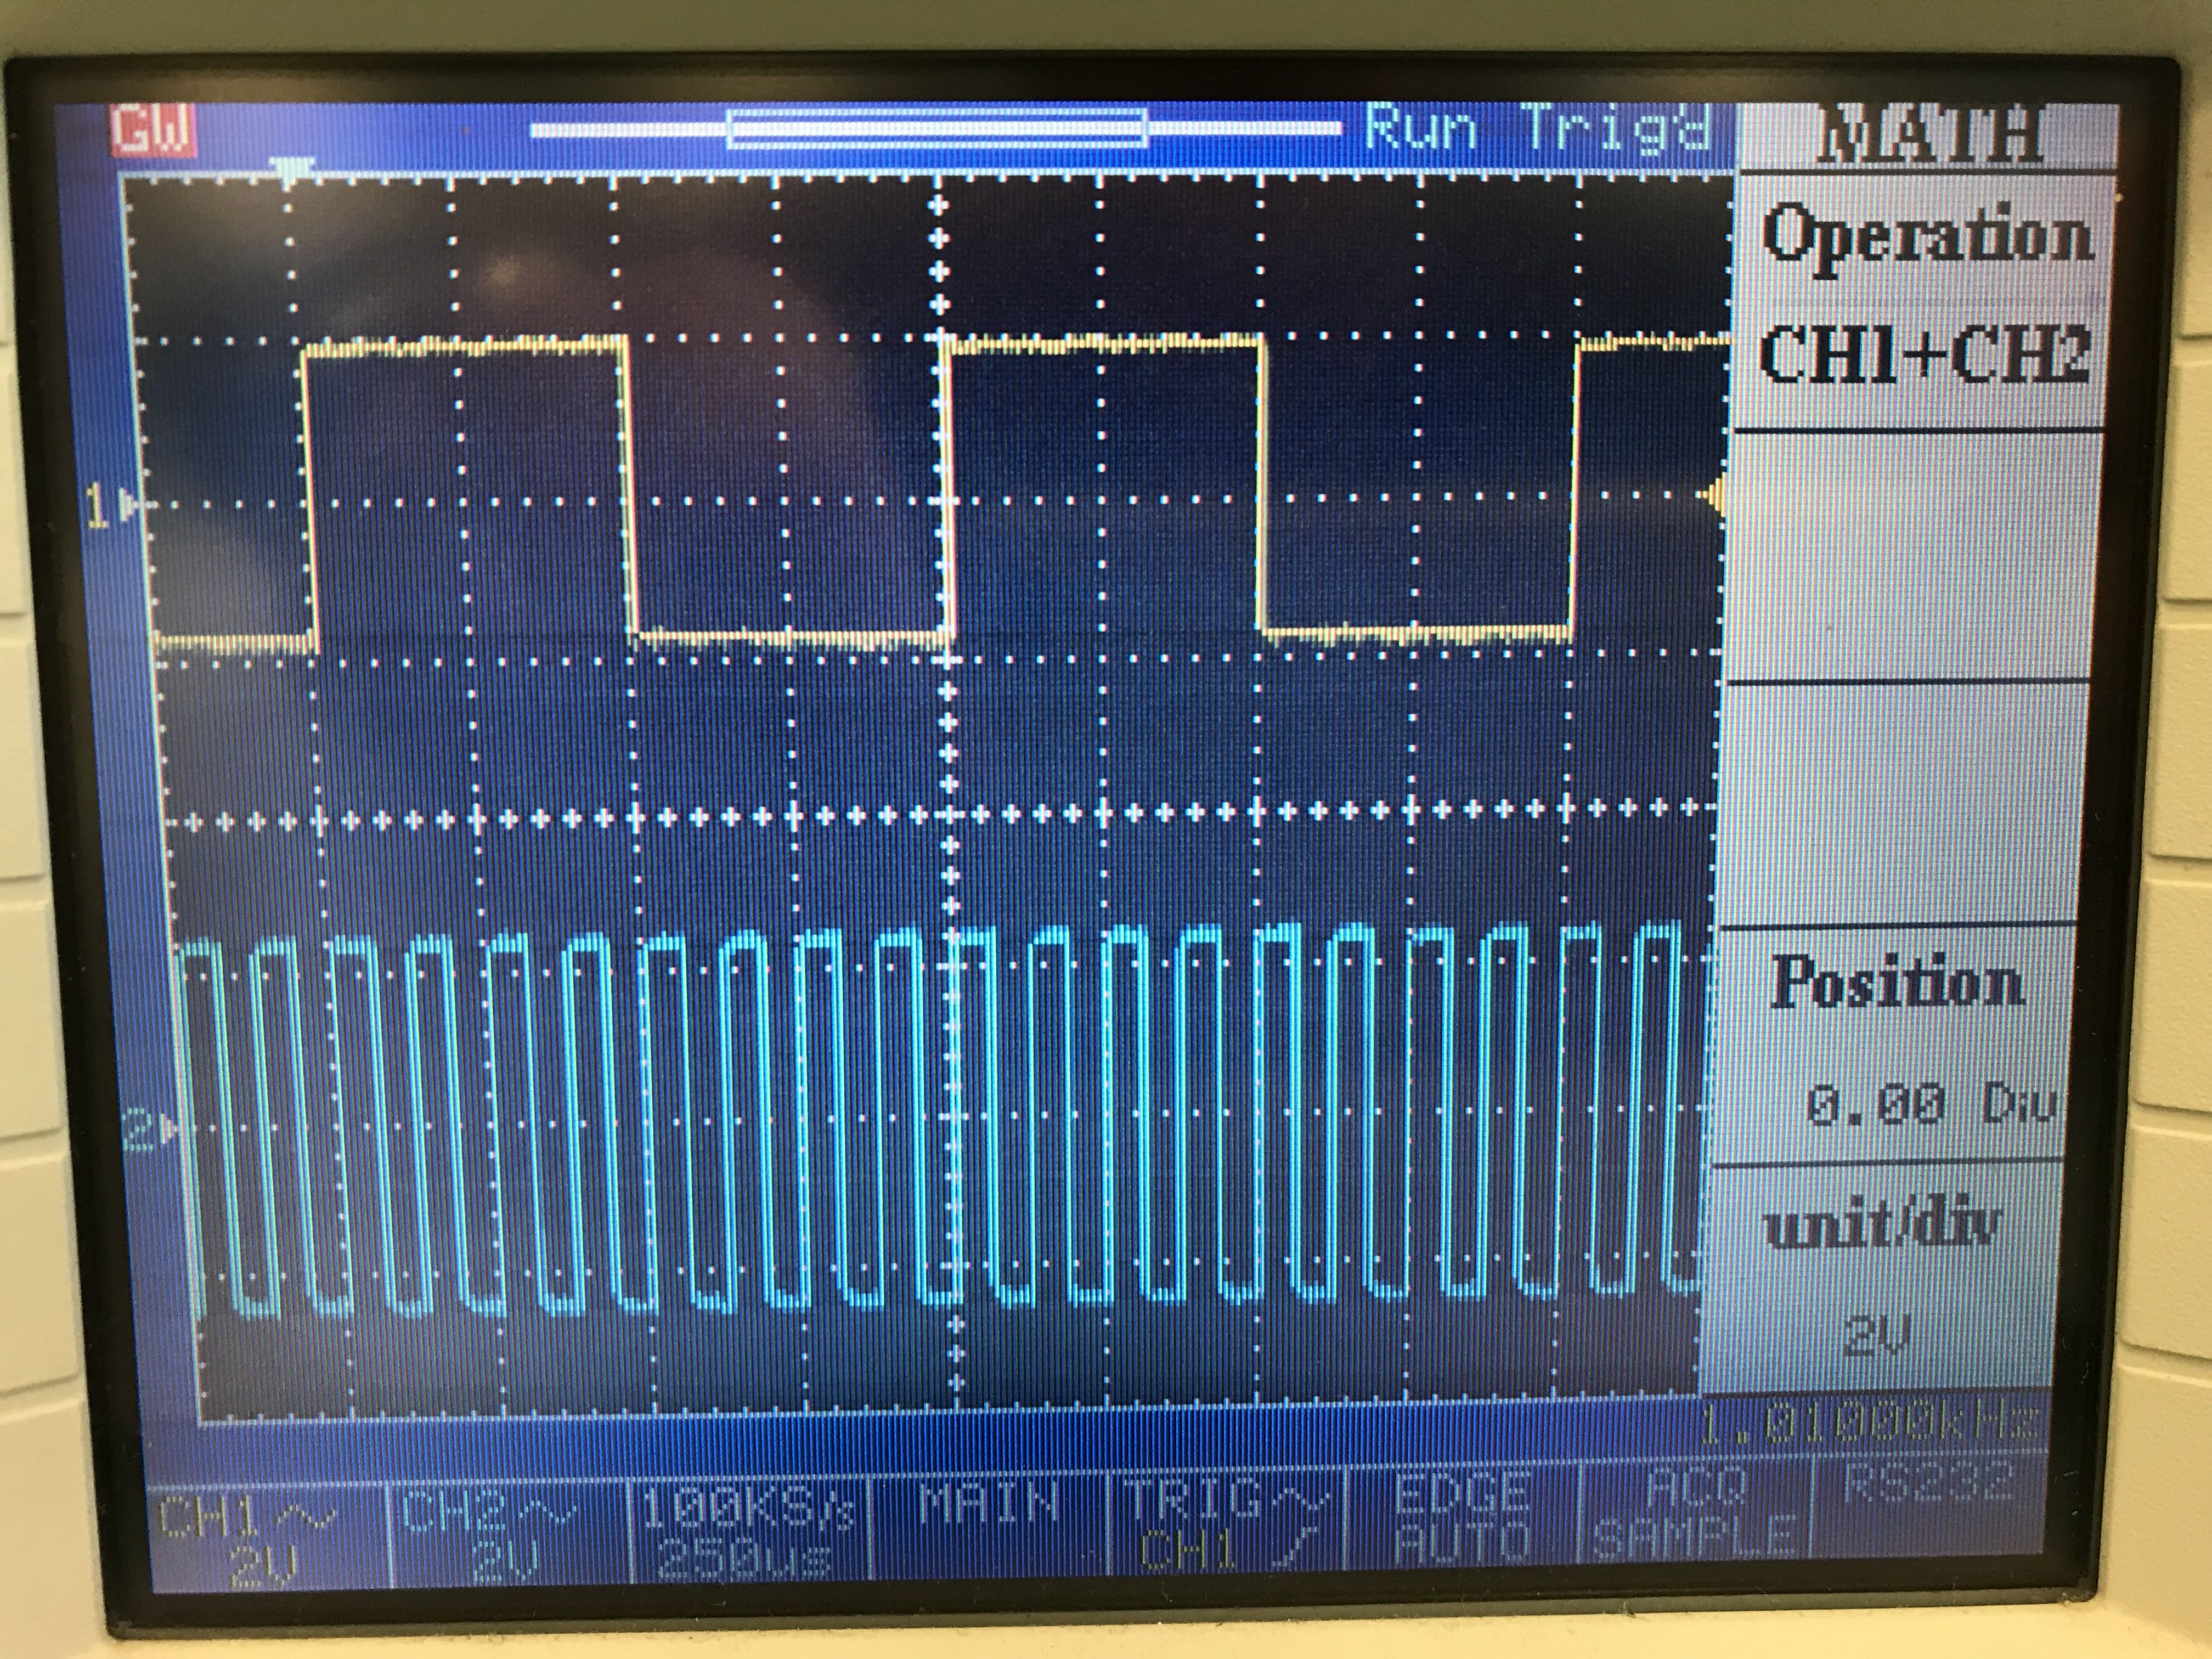
\includegraphics[width=0.5\textwidth]{1over8.jpg}	
	\caption{1/8 frequency of input}
	\label{fig:1over8}
\end{figure}

\newpage
\paragraph{}
In order to produce a signal that has 1/3 pulse-gap ratio, 10001000 bits are loaded to the shift register. This gives a signal that can be seen in Figure \ref{fig:1over3pulsegap} which 
stays in low logic longer than high logic state. It takes 1 cycle from the blue wave to end high logic, however low logic level takes 3 cycles. This concludes that signal is manipulated correctly.
\begin{figure}[h]
	\centering
	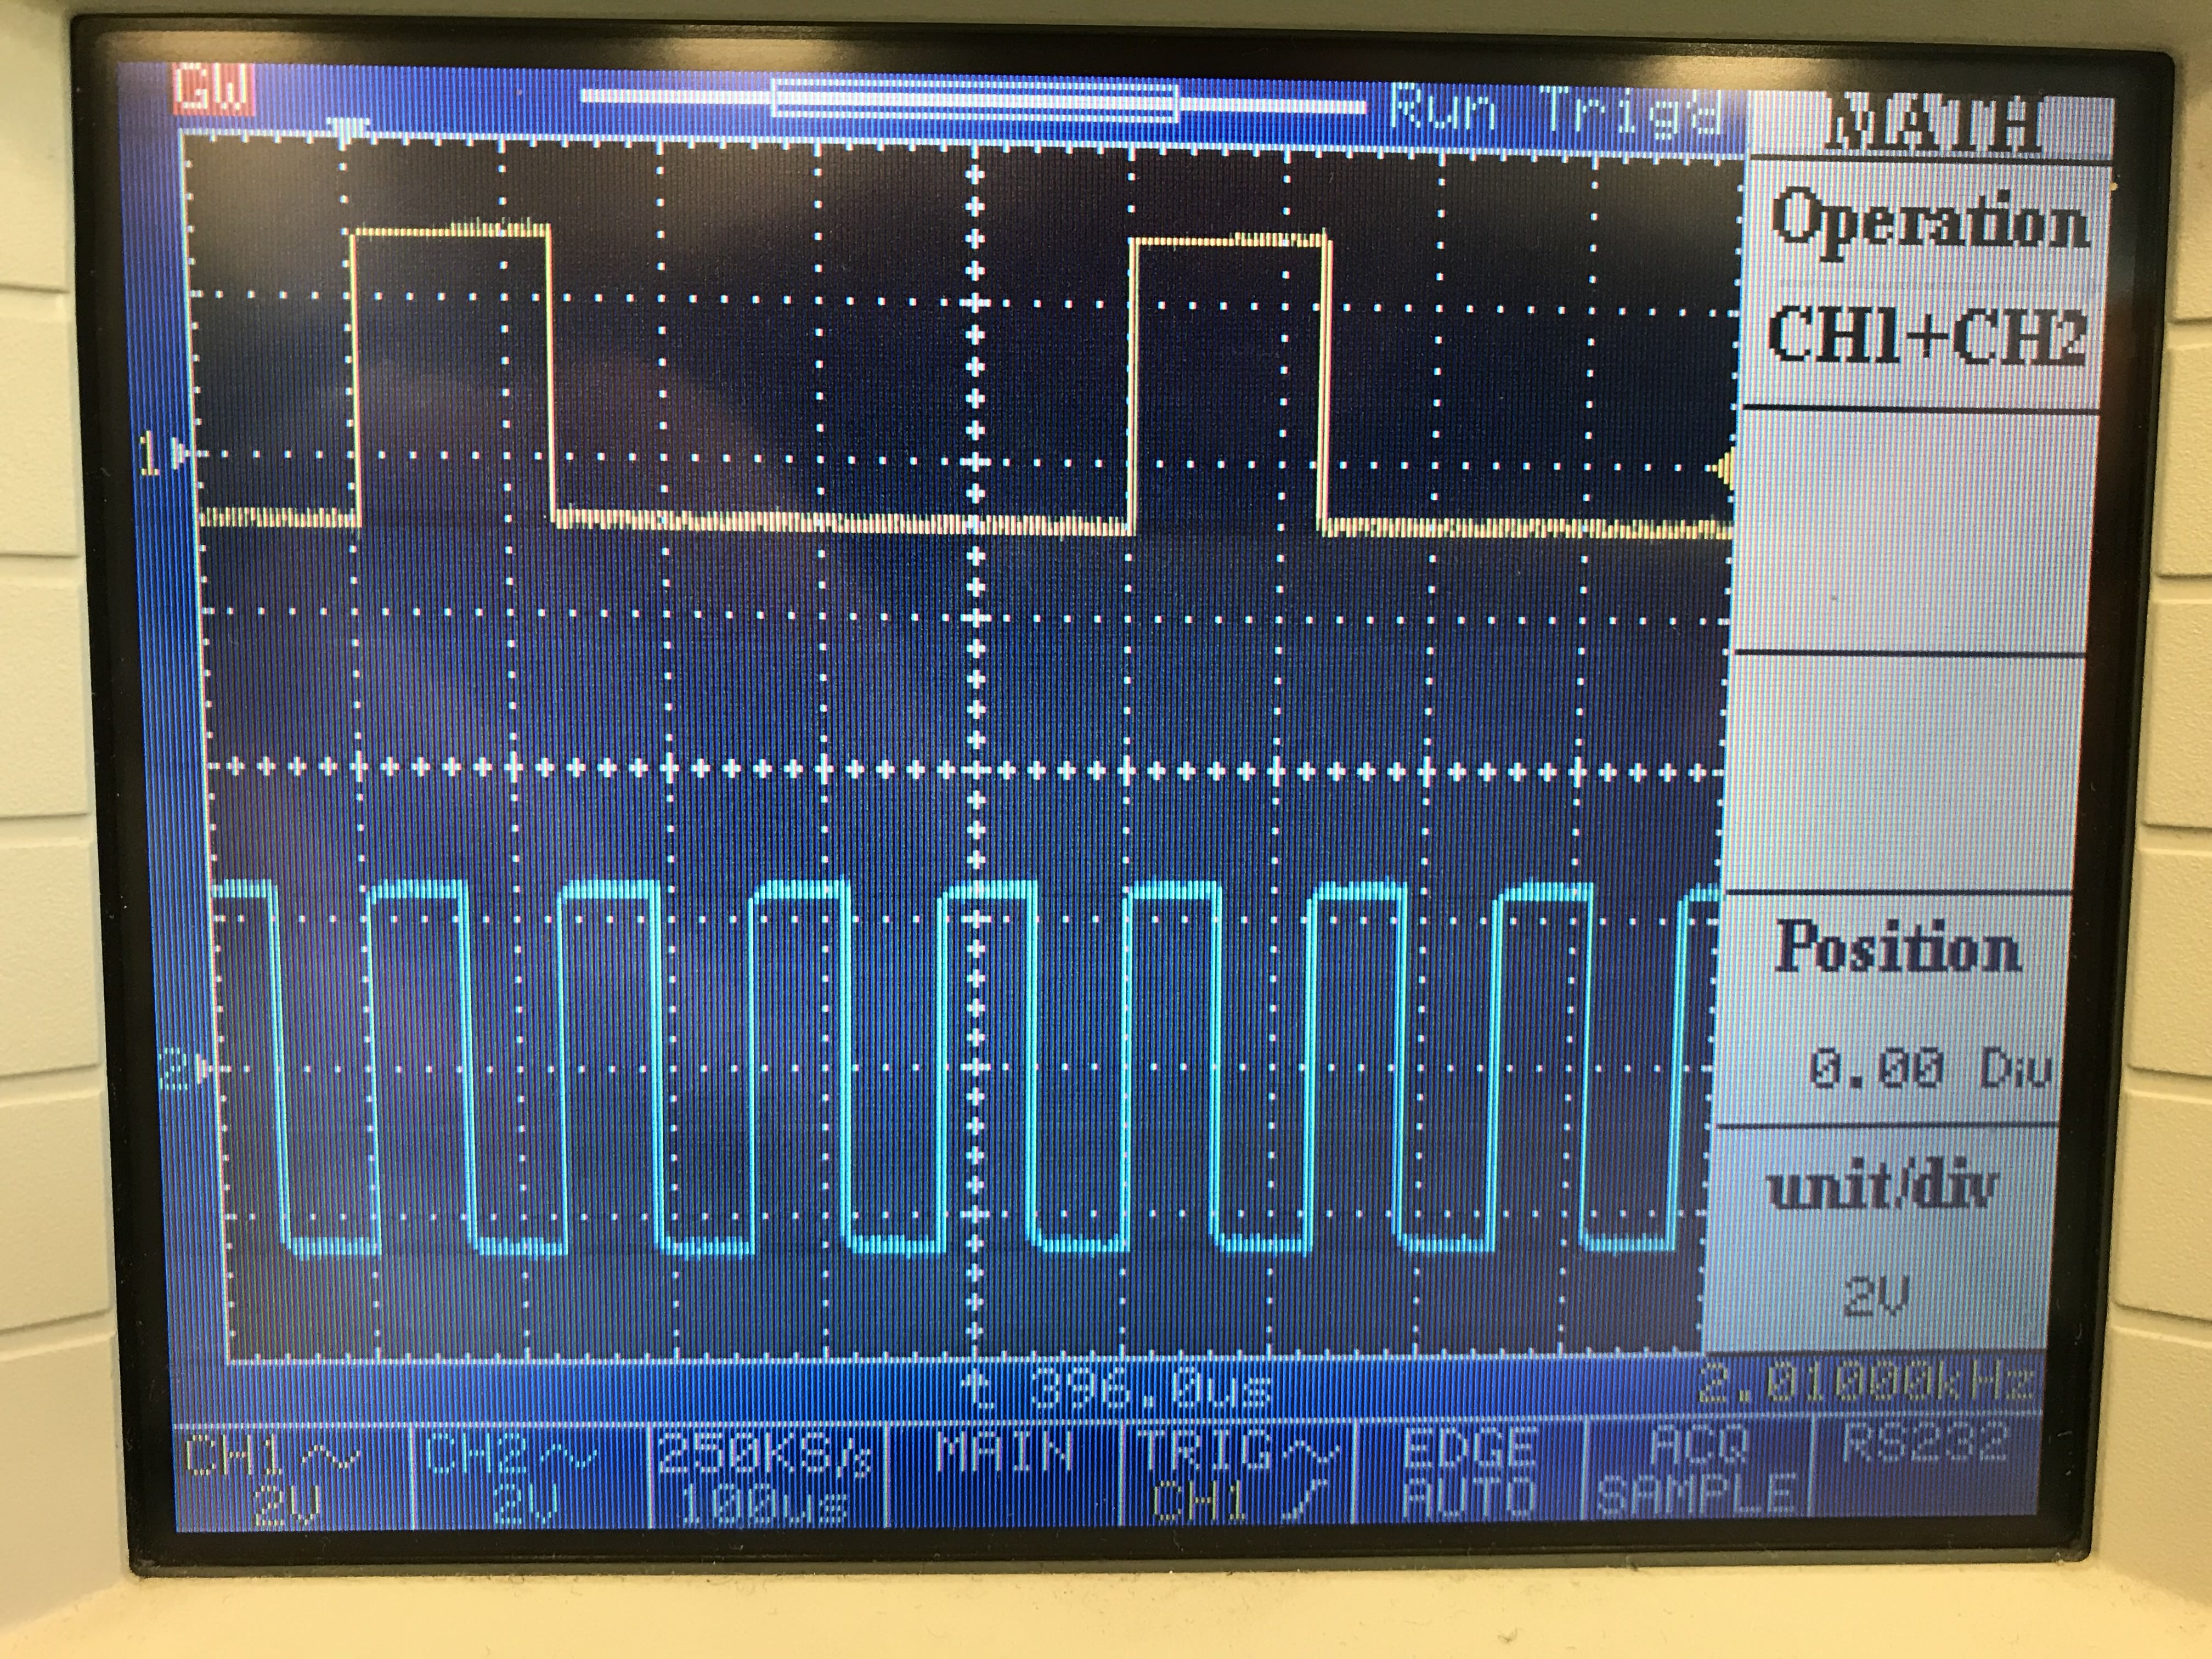
\includegraphics[width=0.5\textwidth]{1over3pulsegap.jpg}	
	\caption{1/3 pulse–gap duration rate}
	\label{fig:1over3pulsegap}
\end{figure}

\paragraph{}
Loading 10000000 bits to the shift register produces the wave in Figure \ref{fig:1over7pulsegap}. This time high level takes 1 cycle and low logic level 7 cycles from the blue wave to complete.
\begin{figure}[h]
	\centering
	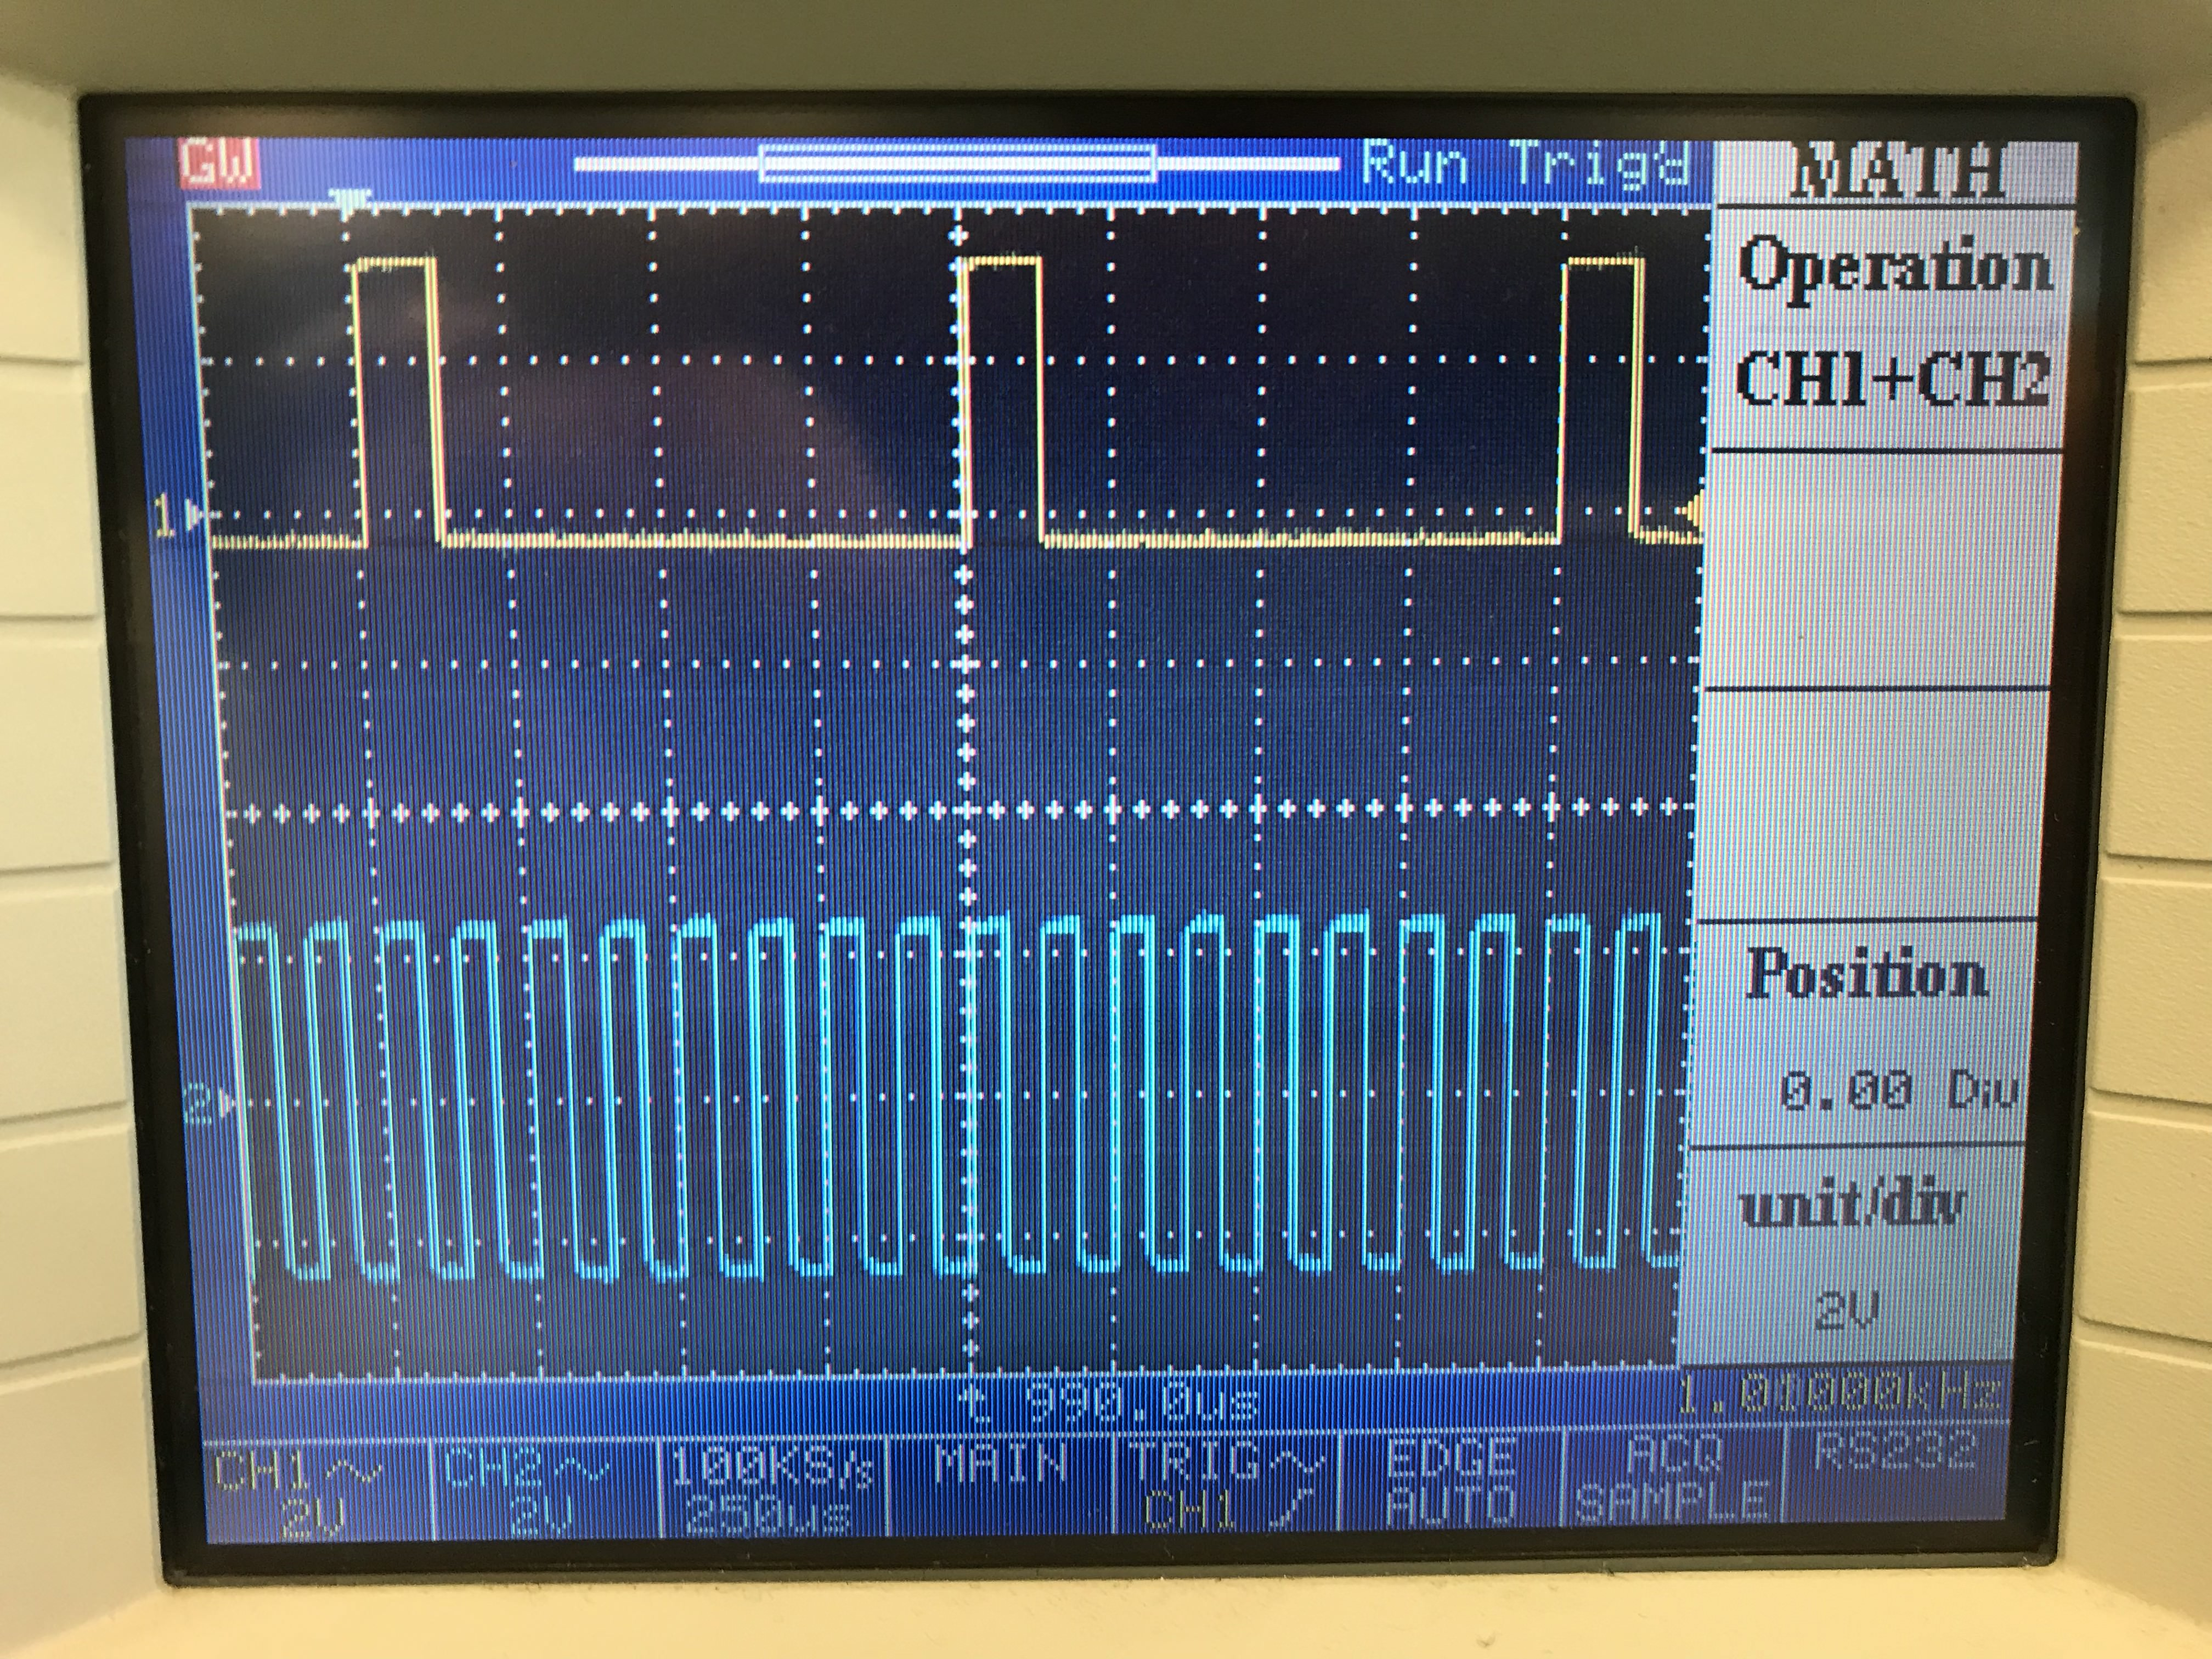
\includegraphics[width=0.5\textwidth]{1over7pulsegap.jpg}	
	\caption{1/7 pulse–gap duration rate}
	\label{fig:1over7pulsegap}
\end{figure}


\end{flushleft}


\newpage
\section{INTERPRETATION OF THE RESULTS}
\begin{flushleft}
\paragraph{}
There weren't any results which contradicted with the theoretical result we have calculated before the experiment. For forbidden inputs, we observed different, unpredictable result which differ because of the different gates used in different circuits as explained above. Also, we have learned that input signal can be manipulated by using a circular shift register.
%yaz gitsin ya ben kaçtım gorusurz yarın yine bi elimine olayım mealy moore da temiz vf
% sonuc cikarmicak miyiz yani burdan input signali manipule edilebildigini gormus olduk yani xd zaten onu yapiyoruz ama onu deneyde soylemedikleri icin cikarim olarak yazialbilir diye dusundum ben
\end{flushleft}

\section{CONCLUSION}
\begin{flushleft}
\paragraph{}
We didn't face any particular difficulties that were worth noting throughout the experiment. We were able to complete the given tasks quite swiftly. All in all, this experiment helped us improve our abilities to implement latches and flip-flops in a multiplicity of different situations.

% savas memes yok mu not today.. not today savaşı kaybettiğimiz bi hikaye anlatmak istemiyorum, grubun çoğunluğu şehit düştü asdaf
\end{flushleft}

\nocite{overleaf}
\nocite{reportGuide}

\newpage


\addcontentsline{toc}{section}{\numberline {}REFERENCES}

\bibliographystyle{unsrt}
\bibliography{reference}

\end{document}

